\section{Objectives}

Manipulation of objects is one the most inherent action of the humankind. Humans never stood and plan about how to manipulate an object. 
It is a natural instict for humans to grab objects in certain ways. Even an infant human can easily manipulate different shapes and colors of objects.
Manipulation helps us to use tools, gadget to achieve tasks and provide service. 
Therefore, manipulation skills will be central for robots of any kind. 
From rehabilitation to service robots, tool usage is vital to enable them to achieve their objective. Our daily manipulation tasks are shown in figure \ref{fig:x manipulation_skills}.
For a complicated manipulation task first of all grapsing the object is essential. We need to first firmly grasp a water bottle to drink it.
Without a firm grasp the safety of the manipulation process is projected to risk. 

Nowadays, every kinds of robots are helping us produce in the industry. However, those robots at the manufacture facilities are only capable of doing same repetitive task. 
The task they are responsible of expands the car manufacturing to high precision microchip producing. On all those tasks robots are extremely efficient and precise. 
On the other hand, if a the car company decides to manufacture a new model of car with a slightly different chasis the whole process needs to be changed and program of the robots needs to be hardcoded from zero.
Hardcoding every move of the robot in a slight change of a task is fundementally opposes the very nature of the robots. 
Main objective of this master's thesis is to enable robotic manipulators to incrementally learn to grasp tools and generalize the learned policy to unseen objects.
Rather than overfitting to a certain set of objects, we measure the success rate on unseen dataset. 
This preassumption promises a robust actor that can adapt well on unseen object and environments.


\begin{figure}[htbp]
    \centering
      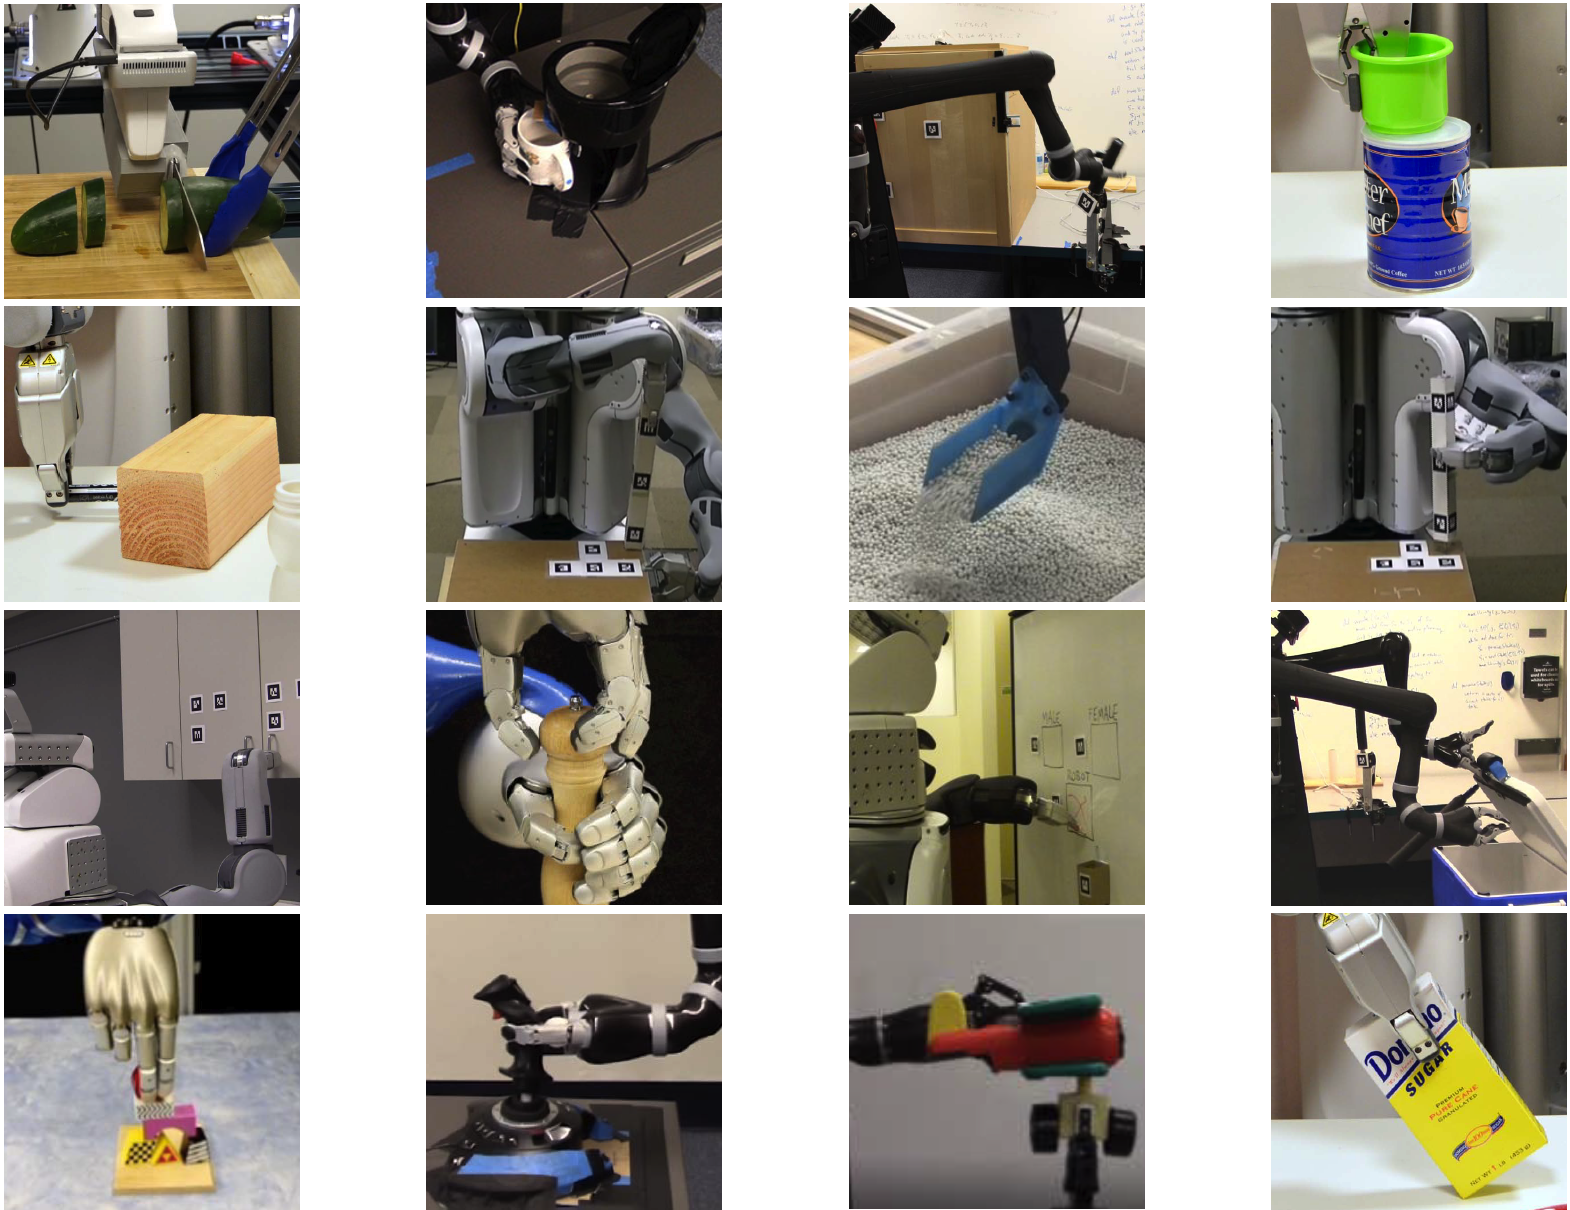
\includegraphics[width=0.8\textwidth]{figures/manipulation_skill}
    \caption{Different manipulation skill adopted to robotic manipulators \cite{Kroemer201}}
    \label{fig:x manipulation_skills}
\end{figure}